%% Hi, people whoerver using theis model. This is Hang Gao. 

%% 您需要知道,本模板按照 吉林大学本科毕业论文 要求,改自 华中科技大学 本科毕业论文模板,该模板由 冯洲 同学创建。原模板中还包括有开题报告,文献综述,外文翻译,请自行适用。

%%本人只是在进行毕业设计的间隙,修改了该模板,为己所用。我很乐意将所修改模板分享给大家,以节省宝贵的时间。所有权利归 冯洲 所有,原项目Copyright (C) 2019~ by Zhou Feng 冯洲 <https://github.com/zfengg>。 

%% 2021年本项在GitHub中地址<https://github.com/Herbert-Gao/JLU_GraduationModel_Bachelor.git>。编辑本文的时间为2021/6 。

%% 将封面按照word格式修改后发表为pdf,然后替换[封面.pdf]文件,即可。



\documentclass[a4paper,twoside]{article}
% 10.5pt equals 5 hao font. 

%----------------------------------------------------------------%
%% For the layout of paper
%\usepackage[tmargin=1in,bmargin=1in,lmargin=1.25in,rmargin=1.25in]{geometry}
\usepackage[top=2.54cm, bottom=2.54cm, left=3.18cm, right=3.18cm]{geometry}
\geometry{headsep=1em,footskip=2em}
\geometry{headheight=14pt}

%----------------------------------------------------------------%
%% For Math Symbols, 载入常用的数学包, 符号包
\usepackage{amsmath}
\usepackage{amsfonts}
\usepackage{amssymb}
\usepackage{mathrsfs}
\usepackage[table,xcdraw]{xcolor}

%----------------------------------------------------------------%
%% For the linespace 行间距,段间距等等
\usepackage{setspace} 
% \usepackage{indentfirst} % then the first line of each title should start with a indent.
% 定义标题和段落样式
% 定义1.5倍行距
\renewcommand{\baselinestretch}{1.62}
\setlength{\baselineskip}{12pt}   % set the fixed value of the lineskip
\setlength\parskip{\baselineskip} % set the space between the paragraphs, set the variable \parskip \baselineskip
% parindent
\setlength{\parindent}{0pt}

%----------------------------------------------------------------%
%% for the fonts (style, color, size).字体的大小,颜色,以及定义常用的字号
\usepackage{ctex}		 	% If you are lazy, the CTEX suit is enough.
% Chinese Font
\usepackage{xeCJK}		 	% For the Chinese through XeLaTex
\setCJKmainfont{FandolSong} 	% set the mainfont of Chinese as songti. (serif) for  
\setCJKsansfont{FandolSong}	% sans serif font for \textsf
\setCJKmonofont{FandolSong}	% monospace font for \texttt
% \punctstyle{kaiming}  	% Remove the space used by symbols like comma. Special for the mainland students like us HUSTers.
\setCJKfamilyfont{song}{FandolSong}                  %宋体 song
\newcommand{\song}{\CJKfamily{song}}                      
\setCJKfamilyfont{kai}{FandolKai}                         %楷体  kai
\newcommand{\kai}{\CJKfamily{kai}}  
\setCJKfamilyfont{hwzs}{FandolFang}                 %华文中宋  hwzs
\newcommand{\hwzs}{\CJKfamily{hwzs}}
\setCJKfamilyfont{hei}{FandolHei}                      %黑体  hei
\newcommand{\hei}{\CJKfamily{hei}}
% English font
\usepackage{fontspec}% Then you can use the fonts installed at your device. 
\setmainfont{Times New Roman}
\setsansfont{Times New Roman}
\setmonofont{Times New Roman}
%\setsansfont{[foo.ttf]} % for the fonts at this default path.
% Font Color 利用definecolor自己可以定义颜色
\usepackage{xcolor}
\definecolor{MSBlue}{rgb}{.204,.353,.541}
\definecolor{MSLightBlue}{rgb}{.31,.506,.741}
% Font Size (I use pinyin represents the corresponding size in Microsorft Word)
% \newcommand{\chuhao}{\fontsize{42pt}{\baselineskip}\selectfont}
\newcommand{\xiaochuhao}{\fontsize{36pt}{\baselineskip}\selectfont}
% \newcommand{\yihao}{\fontsize{28pt}{\baselineskip}\selectfont}
\newcommand{\erhao}{\fontsize{21pt}{\baselineskip}\selectfont}
\newcommand{\xiaoerhao}{\fontsize{18pt}{\baselineskip}\selectfont}
\newcommand{\xiaosanhao}{\fontsize{15pt}{\baselineskip}\selectfont}
\newcommand{\sanhao}{\fontsize{15.75pt}{\baselineskip}\selectfont}
\newcommand{\sihao}{\fontsize{14pt}{18pt}\selectfont}
\newcommand{\xiaosihao}{\fontsize{12pt}{18pt}\selectfont}
\newcommand{\wuhao}{\fontsize{10.5pt}{18pt}\selectfont}
\newcommand{\xiaowuhao}{\fontsize{9pt}{\baselineskip}\selectfont}
% \newcommand{\liuhao}{\fontsize{7.875pt}{\baselineskip}\selectfont}
% \newcommand{\qihao}{\fontsize{5.25pt}{\baselineskip}\selectfont}


%% set the styles of sections at all levels
 %设置各个标题样式
 %不需要使用part和chapter层级
 \usepackage{titlesec}
 \usepackage{titletoc}
 \titleformat{\section}{\centering \hei \bfseries\xiaosanhao}{第\,\thesection\,章}{1em}{} % 在section标题编号后面加个点
% \titlelabel{\thetitle.\quad} % add a dot after the counter for all levels of sections
 \titleformat*{\subsection}{\raggedright \hei \bfseries \sihao}
 \titleformat*{\subsubsection}{\raggedright \hei \xiaosihao}
 \titleformat{\paragraph}[hang]{\raggedright \song \bfseries \xiaosihao}{\theparagraph}{1em}{}[]
 \titleformat{\part}{\centering \hei \bfseries \xiaosanhao}{}{1em}{}

 % Manual
%\titleformat{command}[shape]{format}{label}{sep}{before-code}[after-code]
%\titlespacing{command}{left}{before-sep}{after-sep}
% %设置新的层级subsubsubsection
\setcounter{tocdepth}{4}
\setcounter{secnumdepth}{4}

\newcommand{\sectionbreak}{\clearpage} %小节从新的一页开始
%根据学校要求设置新的section, subsection, subsection,  paragraph

% set the content of section and so on
\newcommand\seccontent{
	\song
	\xiaosihao 
    \setlength{\parindent}{2em} % 首段缩进两个M字符
    \setlength{\parskip}{0pt}
    }
\newcommand\tabcontent{
	\song
	\wuhao % 默认五号字体, 行间距为1.5*\baselineskip
	\setlength{\parindent}{2em} % 首段缩进两个M字符
	\setlength{\parskip}{0pt}
}

%----------------------------------------------------------------%
%% For the header and footer. 页眉,页脚
 \usepackage{fancyhdr} % Then you can specialize the header and footer for your own use.
 % 设置页眉样式
 % 设置标题页的属性

\pagestyle{fancy} % 选用 fancy style
\fancyhf{}
\fancyhead[CE]{吉林大学本科毕业设计(论文) \kai \xiaowuhao}
\renewcommand{\sectionmark}[1]{\markboth{第\,\thesection\,章 \ #1}{}}
\fancyhead[CO]{\leftmark  \kai \xiaowuhao}
\fancyfoot[LE,RO]{~\thepage~}
\renewcommand{\headrulewidth}{0.7pt}


%----------------------------------------------------------------%
%----------------------------------------------------------------%
%% For the style of theorems, definitions, proofs and remarks 定义数学里面一些常用的环境
\usepackage{amsthm}
\newtheorem{thm}{\textbf{定理}}[section]
 %The section in [] can be replaced by chapter or subsection
 \theoremstyle{definition} \newtheorem{law}[thm]{Law}
 \theoremstyle{plain} \newtheorem{jury}[thm]{Jury}
 \theoremstyle{remark} \newtheorem*{marg}{Margaret}

%----------------------------------------------------------------%
%% For the caption and reference 图表及公式的编号规范
\usepackage{float} 		 		  	% table figure positioning
\usepackage{caption}


\captionsetup[figure]{labelformat=default, labelsep=quad,name={图}}
\captionsetup[table]{labelformat=default,labelsep=quad,name={表}}
%设置图表标题的计数方式
\renewcommand{\thefigure}{\ifnum \thesection>0 \thesection.\fi \arabic{figure}} % set caption label style to 2-1 
\renewcommand{\thetable}{\ifnum \thesection>0 \thesection.\fi \arabic{table}} % set caption label style to 2-1 
\DeclareCaptionFont{mylabelfont}{\hei\xiaosihao}
\captionsetup[figure]{font=mylabelfont} 
\captionsetup[table]{font=mylabelfont} 

%设置图表的autoref的格式
\newcommand{\reffig}[1]{图 \ref{#1}}
\newcommand{\reftab}[1]{表 \ref{#1}}

%公式的编号格式
\newcommand{\refeq}[1]{公式(\ref{#1})}
\renewcommand{\theequation}{\arabic{section}.\arabic{equation}}

%\usepackage{subfigure}
\usepackage{graphicx} % To include graphixs 添加图所需的包
\usepackage{booktabs} 
\usepackage{multirow}% To create three line table including the commands toprule, bottomrule, and midrule
%\usepackage{colortbl} % 
%使用tabularx库并定义新的左右中格式
\usepackage{tabularx}
\usepackage{makecell}
\newcolumntype{L}{X}
\newcolumntype{C}{>{\centering \arraybackslash}X}
\newcolumntype{R}{>{\raggedright \arraybackslash}X}

%----------------------------------------------------------------%
%set the style of counters设置计数器
% 设置重新计数的位置
\makeatletter
\@addtoreset{footnote}{page}
\@addtoreset{figure}{section}
\@addtoreset{table}{section}
\@addtoreset{equation}{section}
\makeatother




%----------------------------------------------------------------%
%% 目录 
%\renewcommand\listfigurename{插图列表}
%\renewcommand\listtablename{表格列表} 
%\titlecontents{标题名}[左间距]{标题格式}{标题标志}{无序号标题}{指引线与页码}[下间距]
%\dottedcontents{section}[2.55em]{\song \xiaosihao \bfseries}{2.5em}{1em}
\usepackage{tocloft}
\renewcommand{\contentsname}{\centerline{ \hei\sanhao 目\hspace{2em}录}}
\titlecontents{section}[0em]{\song\xiaosihao}{第\space\space\contentslabel{0em}\hspace{1em}章\quad}{}{\titlerule*[8pt]{.}\contentspage}
\titlecontents{subsection}[4em]{\song\xiaosihao}{\contentslabel{2em}}{\hspace*{-4em}}{\titlerule*[8pt]{.}\contentspage}
\titlecontents{[width=1cm]}[8em]{\song\xiaosihao}{\contentslabel{3em}}{\hspace*{-5em}}{\titlerule*[8pt]{.}\contentspage}
%\titlecontents{paragraph}[5em]{\song\xiaosihao}{\contentslabel{5em}}{\hspace*{-5em}}{\titlerule*[8pt]{.}\contentspage}




%----------------------------------------------------------------%
%% For the bibiliograph or reference and citation 参考文献
\usepackage{gbt7714}
\bibsep=0pt % 用来设置每个\bibitem之间的间距
%\renewcommand{\bibname}{参考文献} % For the document class 参考文献
%\newcommand{\upcite}[1]{\textsuperscript{\textsuperscript{\cite{#1}}}} % If you want the citation label to show at the uperscript position.
%----------------------------------------------------------------%
%设置声明页
%使用特殊符号
\usepackage{amssymb}
\usepackage{wasysym}
%制作tatement中的符号
\def\HUSTcheckedbox{$\Square\!\!\!\!\checkmark$}
\def\HUSTbox{$\Square$}
%设置命令
\newcommand{\statement}[2]{
	\def\yearofconfidentiality{\hspace{2em}}

    \def\HUSTconfidential{\HUSTbox}
	\def\HUSTnotconfidential{\HUSTcheckedbox}
	\ifnum #1<2
		\def\HUSTconfidential{\HUSTcheckedbox}
		\def\HUSTnotconfidential{\HUSTbox}
		\def\yearofconfidentiality{#2}
	\fi
	\clearpage
	\thispagestyle{main}
	\vspace*{1em}
	\seccontent
	\begin{center}
		\heiti \xiaoerhao \bfseries
		学位论文原创性声明
	\end{center}


    本人郑重声明:所呈交的论文是本人在导师的指导下独立进行研究所取得的研究成果。除了文中特别加以标注引用的内容外,本论文不包括任何其他个人或集体已经发表或撰写的成果作品。本人完全意识到本声明的法律后果由本人承担。
	
	\begin{flushright}
		作者签名:\hspace{6em} 年 \hspace{2em} 月 \hspace{2em} 日
	\end{flushright}
	\vspace{4em}
	
	\begin{center}
		\heiti \zihao{-2} \bfseries
		学位论文版权使用授权书
	\end{center}
	
	
    本学位论文作者完全了解学校有关保障、使用学位论文的规定,同意学校保留并向有关学位论文管理部门或机构送交论文的复印件和电子版,允许论文被查阅和借阅。本人授权省级优秀学士论文评选机构将本学位论文的全部或部分内容编入有关数据进行检索,可以采用影印、缩印或扫描等复制手段保存和汇编本学位论文。

    本学位论文属于 1、保密 \HUSTconfidential ,在 \yearofconfidentiality 年解密后适用本授权书。
			
		    \hspace{7em} 2、不保密 \HUSTnotconfidential \hspace{1em}
			。
			
			\hspace{7em} (请在以上相应方框内打``$\checkmark$'')


	
	\begin{flushright}
	作者签名:\hspace{6em} 年 \hspace{2em} 月 \hspace{2em} 日
	
    导师签名:\hspace{6em} 年 \hspace{2em} 月 \hspace{2em} 日
    \end{flushright}	
	\clearpage
}
\newcommand{\makestatement}[2]{\statement{#1}{#2}}



%-------------------------------------------------------------------%
% 定义中英文摘要和致谢环境
%
% 中文摘要环境
\newenvironment{cnabstract}[1]{
	\def \cnkeyword {#1}
	\clearpage

	\phantomsection
	\addcontentsline{toc}{section}{摘要}
	\vspace*{-20pt}
	\begin{center} 
		\heiti \bfseries \xiaoerhao 摘 \hspace{2em} 要 
	\end{center}
	\seccontent
}{  
	\vspace{1em}
	\par\noindent {\hei\sihao \bfseries 关键词:} {\song\xiaosihao\cnkeyword}

}

% 英文摘要环境
\newenvironment{enabstract}[1]{
	\def \enkeyword {#1}
	\clearpage 
	\phantomsection
	\addcontentsline{toc}{section}{Abstract}
	\vspace*{-20pt}
	\begin{center} 
		\bfseries \xiaoerhao Abstract 
	\end{center}
	\seccontent
}{
	\vspace{1em}
	\par\noindent {\sihao\bfseries Key Words: }\ {\song\xiaosihao\enkeyword}
	\clearpage
}

% 定义致谢环境
\newenvironment{thankpage}{
	\clearpage
	\phantomsection
	\addcontentsline{toc}{section}{致谢}
	\section*{致\hspace{2em}谢}
}{
	\clearpage
}


%---------------------------------------------------------------%
%	---	定义列表项,列举的样式
\usepackage{enumitem}
\setlist{noitemsep}

%----------------------------------------------------------------%
%\usepackage{makeindex} For the index 索引
\usepackage{listings} % For the code. 代码
\usepackage{algorithm}  
\usepackage{algpseudocode}  
\usepackage{amsmath}  
\renewcommand{\algorithmicrequire}{\textbf{Input:}}  % Use Input in the format of Algorithm  
\renewcommand{\algorithmicensure}{\textbf{Output:}} % Use Output in the format of Algorithm  
%---------------------------------------------------------------%
% 设置脚注

%----------------------------------------------------------------%
%% For the hyperlink and bookmark 超链接及书签,(这样生成的pdf中的引用直接点击链接即可到达目的地)
\usepackage[bookmarks=true,colorlinks,linkcolor=black,citecolor=black,urlcolor=purple]{hyperref}% 设置超链接并修改风格


%----------------------------------------------------------------%
%% For the appendix, 附录
% 设置附录
\usepackage{appendix}
\renewcommand{\appendixname}{附录}

%----------------------------------------------------------------%
% For the titlepage 标题页,此处可以省略,建议直接使用官方给出的标题页即可
\usepackage{titling} 
\usepackage{pdfpages}
%重置命令maketitle
\renewcommand{\maketitle}{
	\def\HUSTtitlelength{12em}
 	\begin{titlepage}
		\begin{center}
			\vspace*{0em}
			
\includegraphics[height=2cm]{JLU_bachelor/fig/JLU_logo.jpeg}\\
%			
			\vspace*{4em}
%			
			{\xiaochuhao \hwzs \bfseries 本科生毕业设计[论文]}\\
%			
			\vspace*{6em}
			{\erhao \hei \bfseries \thetitle}
			
			\vspace*{6em}
			{\sanhao \hwzs 
				\renewcommand\arraystretch{2.7}
				\begin{tabular}{lc}
					\makebox[4em][s]{院 \hfill 系} &
					\underline{\makebox[\HUSTtitlelength]{\school}} \\
					\makebox[4em][s]{专业班级} &
					\underline{\makebox[\HUSTtitlelength]{\classnum}} \\
					\makebox[4em][s]{姓 \hfill 名} &
					\underline{\makebox[\HUSTtitlelength]{\theauthor}} \\
					\makebox[4em][s]{学 \hfill 号} &
					\underline{\makebox[\HUSTtitlelength]{\stunum}} \\
					\makebox[4em][s]{指导教师} &
					\underline{\makebox[\HUSTtitlelength]{\instructor}} \\
			  \end{tabular}
		    }
	    
			\vspace{4em}
			{\sanhao \hwzs \thedate}
			
		\end{center}
	\end{titlepage}
}

% ------------titlepage-----------------%
% 下面填写自己相应的信息就可以了
\title{基于贝叶斯非参数方法的驾驶行为分析}  		 % 论文题目
\def\school{汽车工程学院}  	% 院系
\def\classnum{车辆工程151703班}  % 专业班级
\author{郜航}					% 姓名
\def\stunum{15170336} 	  % 学号
\def\instructor{曲婷}			% 指导老师
\date{\today}   			  % 日期,自己填就可以了

%-------------quickinput----------------%
% 利用\newcommand{cmd}{def} 设置一些常用的代码,提高效率,这里可以自行删除,下面是我敲翻译时候打的一些command。
\newcommand{\hongzifuzhu}[1]{\textcolor{red}{\kai \wuhao(#1)}}


\begin{document}

\includepdf[pages={1}]{封面.pdf}
 % 生成标题页,个人建议直接使用学校给的word转成pdf与这里生成的pdf第一页合并,再去打印封皮。
% \thispagestyle{empty}% 标题页不参与编号
%-------------------------------------声明页--------------------------------%    
\clearpage
\thispagestyle{empty}
\vspace*{1em}
\seccontent
\begin{center}
	\heiti \xiaoerhao \bfseries
	吉林大学学士学位承诺书
\end{center}

~\\
本人郑重承诺:所呈交的学士学位毕业论文(设计),是本人在指导教师的指导下,独立进行实验、设计、调研等工作基础上取得的成果。除文中已经注明引用的内容外,本论文(设计)不包含任何其他个人或集体已经发表或撰写的作品成果。对本人实验或设计中做出重要贡献的个人或集体,均已在文中以明确的方式注明。本人完全意识到本承诺书的法律结果由本人承担。

~\\








\begin{flushright}
	承诺人:
	\hspace{6em} 年 \hspace{2em} 月 \hspace{2em} 日
\end{flushright}
\vspace{4em}
%---------------------------------------中文摘要----------------------------%
\clearpage
\setcounter{page}{1}
\renewcommand{\thepage}{\Roman{page}}

\begin{cnabstract}{非参贝叶斯;HDP-HMM,sticky HDP-HMM,HDP-HSMM;跟驰工况;K-means;驾驶风格语义;礼让性与鲁莽性}
	\hspace{2em}
驾驶员的驾驶行为能够显著影响车辆行驶的油耗和道路安全。无人驾驶汽车的到来又使得关于驾驶员模型的研究受到广泛关注。过去驾驶员模型是基于智能控制理论建立的,近年来出现了利用机器学习方法建立的驾驶员模型。

本文基于非参贝叶斯模型方法,将时间序列划分为不同的时间片段,对应赋予其驾驶模式特征,进而通过统计学分析得到具有语义的驾驶风格。在分析过程中,使用了HDP-HMM,sticky HDP-HMM和HDP-HSMM三种算法对时间序列进行分割,通过比较得出HDP-HSMM算法在跟驰工况下表现最优的结论。划分时间序列后,使用K-means聚类对时间片段进行聚合,并且按照阈值标注。将标注结果按照相对距离划分为远距离,中距离和短距离三种,得到三张相对速度-加速度频率分布图,反映出驾驶风格。本分析结果还可以用来判断驾驶行为的礼让性和鲁莽性。

最终,通过比较不同驾驶员的分析结果,得到了“驾驶员行驶过程中礼让程度不会因为跟驰距离的远近而改变”,“在远距离跟驰的情况下,各驾驶员表现出来的驾驶风格差异不大”等结论。
\end{cnabstract}

%---------------------------------------英文摘要----------------------------%
\begin{enabstract}{non-parametric Bayesian model;HDP-HMM,sticky HDP-HMM,HDP-HSMM;car-following;K-means;semantic driving style;driving comity and recklessness}

Driving style can significantly affect the fuel consumption and road safety of the vehicle. Besides, The arrival of driverless cars has brought widespread attention to the research on driver models. In the past, driver models were based on intelligent control theory. In recent years, driver models based on machine learning have emerged.

This article uses the non-parametric Bayesian model to divide the time series into different driving modes. Then the semantic driving style through statistical analysis is obtained. In the analysis process, three algorithms of HDP-HMM, sticky HDP-HMM and HDP-HSMM are used to segment the time series. The conclusion that the HDP-HSMM algorithm performs best under car-following conditions is obtained through comparison. After partitioning, K-means clustering is used to aggregate the time segments and label them according to the threshold. Divide the labeling results according to the relative distance, and get the relative speed-acceleration frequency distribution map. After that, we can get the driver's driving style. The results of this analysis can also be used to judge the driver's driving comity and recklessness. 

Finally, by comparing the analysis results of different drivers, it is obtained that "drivers' degree of driving comity will not change due to the relative distance of the cars " , "there is little difference in driving style in the case of long-distance car following. " and some other conclusions.
\end{enabstract}


\vspace*{-1em}
\tableofcontents


\clearpage
\setcounter{page}{1}
\renewcommand{\thepage}{\arabic{page}}


%------------------------------------主体内容--------------------%   
\seccontent


\section{绪论}
\subsection{研究背景}



\subsubsection{驾驶员模型简介}


\subsubsection{无人驾驶技术发展现状}%无人驾驶汽车简介


\subsubsection{驾驶风格研究现状}%后部分研究方向介绍,文章testing.pdf[8],[9]


\subsection{驾驶风格研究现状和总结}%国内外发展介绍后部分,前部分研究方向介绍,研究进展情况


\subsection{研究意义}\label{sec:youhao}



\subsection{总体研究思路及方案}%总的intro

\section{非参贝叶斯相关算法}
本文研究过程中涉及了多个算法,其中利用的知识包含了概率论,线性代数等数学知识。现就其中涉及的算法核心进行解释,相关基础知识可见于附录中。
\subsection{狄利克雷过程}

\subsection{马尔科夫链}


\subsection{马尔科夫模型的推广}


\section{数据收集与前期处理}

\begin{algorithm}[H]
  \caption{从SPMD数据集中提取广义跟驰工况}  
  \label{alg:carfollowing}  
  \begin{algorithmic}  
    \Require  
    DataFrontTargets,  DataWsu \textbf{in} SPMD
    \Ensure  
   CarFollowingSeq2
    \For{$\quad r_t$ \textbf{in} DataFrontTargets$\quad s_t$ \textbf{in} DataWsu $\quad$}
        \State \textbf{add} $f_t={r_t \cup s_t}$ \textbf{to} CarFollowingSeq1;
        \If{$CIPV_t=1 \quad \& \quad TargetType_t=0 \quad \& \quad  ObstacleId_t=ObstacleId_{t-1}$ \textbf{in} $f_t$}
            \State \textbf{add} $g_t=f_t$ \textbf{to} CarFollowingSeq2;
        \EndIf
    \EndFor
  \end{algorithmic}  
\end{algorithm}



\subsection{跟驰工况定义及要求}

\subsection{时间序列分割}


\subsubsection{分割过程}


\subsubsection{评价指标}\label{sec:one_person}


\subsection{分割结果聚类}


\subsection{按照阈值划分}


\subsection{分析结果表示}\label{sec:one_event}


\subsubsection{多个驾驶员驾驶风格对比}

\subsection{思考与讨论}

\subsubsection{时间序列划分及聚类的意义}

\subsubsection{研究结合实例}\label{sec:kongzhiqi}

\section{工程管理与社会}

\subsection{驾驶风格与行车安全之间联系}

\subsection{驾驶风格与自然环境之间联系}

\section{工作总结}



%-----------------------致谢---------------------------------------%
\begin{thankpage}

\end{thankpage}


%-------------------------参考文献----------------------------------%
\clearpage
\addcontentsline{toc}{section}{参考文献}

\bibliography{reference}


%----------------------------附录----------------------------------%
\clearpage
\appendix
\part{附录}
附录内容包括对本文中用到的与算法相关知识的补充、文章内容中提到证明过程、英文原稿和中文翻译。
\subsection*{算法的相关知识}
\subsubsection*{伽马函数及其分布}
伽马分布是统计学中的常用到的一种连续概率函数,又可以记为$\Gamma$分布。它是指数分布和$\chi^2$分布的普遍形式。

伽马函数的表达式可以表示为
$$\Gamma(\alpha)=\int_{0}^{\infty} t^{\alpha-1} e^{-t} d t
$$
若对$t$做积分变换$t=\beta x$,可以得到
$$
\Gamma(\alpha, \beta)=\beta^{\alpha} \int_{0}^{\infty} x^{\alpha-1} e^{-x \beta} d x
$$
其中,$\alpha$称为形状参数,$\beta$称为逆尺度参数。\\
可以通过分部积分的方法,推导出函数具有以下递归性质,
$$
\Gamma(x+1)=x \Gamma(x)
$$
由此可得到,伽马函数与贝塔函数之间的关系为
$$
B(m, n)=\frac{\Gamma(m) \Gamma(n)}{\Gamma(m+n)}
$$
利用伽马函数,可以得到伽马分布的概率密度表达式为
$$
f(x, \beta, \alpha)=\frac{\beta^{\alpha}}{\Gamma(\alpha)} x^{\alpha-1} e^{-\beta x}, x>0
$$
画出概率密度分布图得到
\begin{figure}
    \centering
    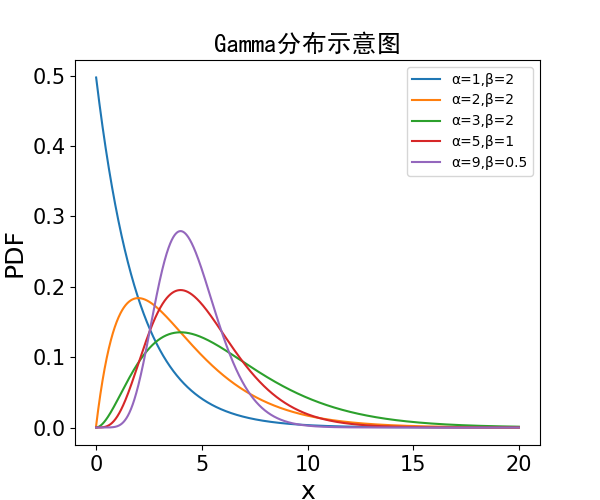
\includegraphics[width=8cm]{JLU_bachelor/appendix_fig/gamma.png}
    %\caption{伽马函数概率密度图}
    \label{fig:gamma}
\end{figure}

\subsubsection*{中餐馆过程}
中餐馆过程可以这样描述:这里有一个中国餐馆,餐馆里有无数张桌子。来吃饭的第一个顾客选择第一个张桌子。对于后来的每一个来到这个餐馆的顾客,按照桌子上人数的比例进行就坐。由于中国人喜欢热闹,自然喜欢坐在人多的桌子上。
第n个顾客选择坐在已经有人的某张桌子上的概率为
$$
p(n,K)=\frac{n_{k}}{\alpha_{0}+n-1}
$$
其中,$K$为已经有顾客桌子的数量,$n_k$为坐在第$k$张桌子上的人数。$\alpha_0$为超参数,决定了每个人坐在新桌子上的喜厌程度。

第n个顾客选择坐在一张新的桌子上的概率为
$$
p(n,K)=\frac{\alpha_{0}}{\alpha_{0}+n-1}
$$

\begin{figure}[H]
    \centering
    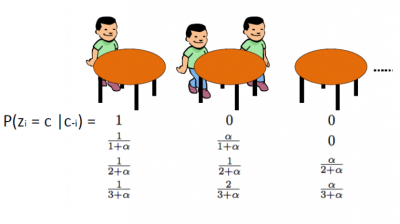
\includegraphics{JLU_bachelor/appendix_fig/chinese.png}
    %\caption{Caption}
    \label{fig:chinese}
\end{figure}

人数越多,就坐在该桌子上的概率就越大。每天中,第一个顾客就坐后,后来的客人会选择坐哪张桌子,共新占了几张桌子,是不确定的。可以通过重复取样来模拟该过程。

可以假设每个顾客坐在某张桌子上的概率服从高斯分布。每一个顾客选择坐在哪张桌子上的过程就相当于是一次从高斯分布中取样的过程。对于第一个顾客,当然会选择坐在概率最大的桌子上,即第一张桌子。在n个顾客选择完桌子后,进行了n次取样。将高斯分布的横坐标等间隔划分为$\alpha_0+1$份,若将每份视为一张桌子,在每份中取样的次数记为坐在该桌子上的人数,就可以模拟每天顾客选择坐桌子上的过程。
\begin{figure}[H]
    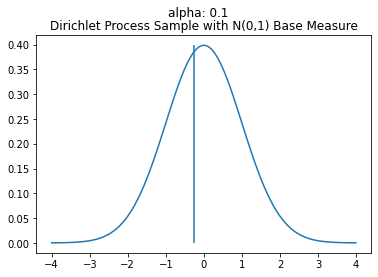
\includegraphics[width=7cm]{JLU_bachelor/appendix_fig/dping1.png}
    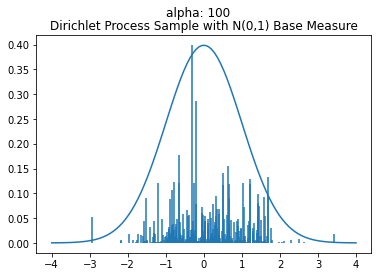
\includegraphics[width=7cm]{JLU_bachelor/appendix_fig/dipping2.png}
    %\caption{狄利克雷取样过程}
    \label{fig:dirich_process}
\end{figure}
以上模拟顾客选择坐位的过程就是狄利克雷过程,取样后划分结果得到顾客的分布情况即狄利克雷分布。
\subsubsection*{GEM过程(Stick Breaking Process)}
除了中餐馆问题模型,还可以将狄利克雷过程描述为将一根完整的棍子折成n段的过程。具体的描述如下:

有一根长度为1的棍子(Stick):
\begin{enumerate}
    \item 截取这根棍子长度为$\beta_1$的一段,并令一个数$\pi1=\beta_1$。则棍子剩下的长度为$L_1=1−\beta_1$;
    \item 截取这根棍子长度为$L_1\beta_2$的一段,并令一个数$\pi_2=L_1\beta_2$。则棍子剩下的长度为$L_2=L_1(1−\beta_2)$;
    \item 截取这根棍子长度为$L_2\beta_3$的一段,并令一个数$\pi_3=L_2\beta_3$。则棍子剩下的长度为$L_3=L_2(1−\beta3_)$;
    \item \dots
\end{enumerate}
可以画出下图来帮助理解:
\begin{figure}[H]
    \centering
    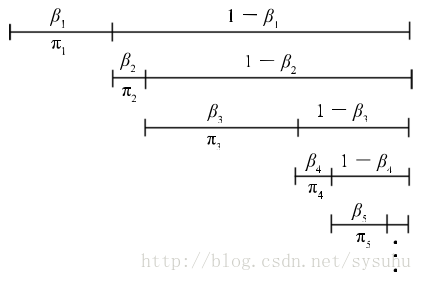
\includegraphics[width=8cm]{JLU_bachelor/appendix_fig/sticks.png}
    %\caption{Caption}
    \label{fig:sticks}
\end{figure}

若定义变量$\beta_i$满足$\beta_i\sim Beta(1,\alpha)$,则根据贝塔分布的性质,$0<\beta_i<1,(i=1,2,\dots)$。引入变量$\beta_0=0$,则可以总结变量$\pi_i$与$\beta_i$之间的关系为
$$
\pi_{i}=\beta_{i} \prod_{i=0}^{i-1}\left(1-\beta_{i}\right)
$$
把这根棍子不断折下去,可以得到很多个$\pi_i$,而且很容易知道有$\sum_{i=1}^{\infty} \pi_{i}=1$。在此过程中,产生的变量$\pi_i$可以看做是关于正整数的随机概率分布。可以理解为:抽样出正整数1的概率为$\pi_1$,抽样出正整数2的概率为$\pi_2$,\dots,抽样出正整数i的概率为$\pi_i$。那么,可以记该过程产生的变量服从分布$\pi_i \sim GEM(\alpha)$。

已知一个分布函数H,定义一个序列$\Phi_1,\Phi_2,\dots$,
其中的每个元素由从分布H中抽样得到,即$\Phi_i \sim H$。假设$\delta \Phi_i$是$\Phi_i$点的概率测度
可以理解为在分布H中抽样得到$\Phi_i$附近的点的可能性的大小。

基于以上,定义一个概率分布:
$$
G=\sum_{i=1}^{\infty} \pi_{i} \delta_{\phi_{i}}
$$
可以认为在分布G中,采样到点$\Phi_1,\Phi_2,\dots$概率分别为$\pi_1\Phi_1,\pi_2\Phi_2,\dots$,
可以证明如此构造的分布函数G是服从狄利克雷过程的,即:
$$G\sim DP(\alpha,H)$$
\subsubsection*{逆威沙特分布}
威沙特分布是用来描述多元正态样本的协方差矩阵而引入的矩阵型随机分布,注意它是一个随机矩阵,不是随机变量。

最简单的Wishart分布:假设有m个独立同分布的$z_{i} \sim N_{p}\left(0, I_{p}\right)$,也就是标准多元正态分布,$V=\sum_{i=1}^{m} z_{i} z_{i}^{\prime}$  ,则称V服从自由度为m的威沙特分布,记做$V\sim W_p(m)$

复杂的威沙特分布:假设有m个独立同分布的$z_{i} \sim N_{p}(0, \Sigma)$   ,也就是中心化的多元正态分布,$W=\sum_{i=1}^{m} z_{i} z_{i}^{\prime}$,则$W\sim W_p(m,\Sigma)$ ,多了一个用于描述多元正态分布协方差阵的参数$\Sigma$。

另一种定义方式:
$$
W \sim W_{p}(m, \Sigma) \quad \quad W=A V A^{\prime}, \Sigma=A A^{\prime}, V \sim W_{p}(m)
$$

威沙特分布和样本协方差阵的关系: 设n个独立同分布的:$x_i\sim N_p(\mu,\Sigma)$,有统计量$$\bar{x}=\frac{\sum_{i=1}^{n} x_{i}}{n}$$ $$S=\frac{1}{n-1} \sum_{i=1}^{n}\left(x_{i}-\bar{x}\right)\left(x_{i}-\bar{x}\right)^{\prime}$$ 那么他们的分布是$$\bar{x} \sim N_{p}\left(\mu, \frac{\Sigma}{n}\right)$$ $$(n-1) S \sim W_{p}(n-1, \Sigma)$$且二者独立。 

逆威沙特分布: 如果一个正定矩阵$B$的逆矩阵  $B^{-1}$服从威沙特分布$W_p(m,\Sigma)$,那么称服从逆威沙特分布$W_p^{-1}(m,\Sigma)$。

逆威沙特分布常作为贝叶斯中多元正态分布的协方差阵的共轭先验分布。假设独立同分布的
$$x_{i} \sim N_{p}(0, \Sigma), \quad \Sigma \sim W_{p}^{-1}(m, \Omega)$$
那么后验条件分布
$$\Sigma \mid data \sim W_{p}^{-1}(m+n, A+\Omega)$$ $$\quad A=\sum_{i=1}^{n} x_{i} x_{i}^{\prime}=n S$$
\subsubsection*{KL散度}
KL散度又称为相对熵。知道了信息熵可以表达数据的信息量大小,是信息处理一个非常重要的概念。\\
对于离散型随机变量,信息熵公式如下:
$$
H(p)=H(X)=\mathrm{E}_{x \sim p(x)}[-\log p(x)]=-\sum_{i=1}^{n} p(x) \log p(x)
$$
对于连续性随机变量,信息熵公式如下:
$$
H(p)=H(X)=\mathrm{E}_{x \sim p(x)}[-\log p(x)]=-\int p(x) \log p(x) d x
$$

相对熵,又被称为KL散度或信息散度,是两个概率分布间差异的非对称性度量 。在信息论中,相对熵等价于两个概率分布的信息熵的差值,若其中一个概率分布为真实分布,另一个为理论(拟合)分布,则此时相对熵等于交叉熵与真实分布的信息熵之差,表示使用理论分布拟合真实分布时产生的信息损耗 。\\
其公式为:
$$
D_{K L}(p \| q)=\sum_{i=1}^{N}\left[p\left(x_{i}\right) \log p\left(x_{i}\right)-p\left(x_{i}\right) \log q\left(x_{i}\right)\right]
$$
上面的$p(x_i)$为真实事件的概率分布,$q(x_i )$为理论拟合出来的该事件的概率分布。

假设理论拟合出来的事件概率分布跟真实的一模一样,那么它就等于真实事件的信息熵,这一点显而易见。

假设拟合的不是特别好,那么它会比真实事件的信息熵大。

也就是在理论拟合出来的事件概率分布跟真实的一模一样的时候,相对熵等于0。而拟合出来不太一样的时候,相对熵大于0。这个性质很关键,因为它正是深度学习梯度下降法需要的特性。假设神经网络拟合完美了,那么它就不再梯度下降,而不完美则因为它大于0而继续下降。

\clearpage
\subsection*{文献翻译}
\subsubsection*{英文原文}


\clearpage
\subsubsection*{翻译内容}


\end{document}